\section {Sprint para Ajustes na Ferramenta de Cadastro de Usuários}

O fluxo de trabalho contou com quatro \textit{sprints} dedicadas para realização do desenvolvimento sobre a ferramenta de textos participativos.
Uma quinta \textit{sprint} foi dedicada unicamente para resolução do problema de desempenho no cadastro de usuários na plataforma. O único requisito da \textit{sprint} é descrito como:

\begin{itemize}
  \item \textbf{Requisito 1 da Sprint}: Resolver o problema de lentidão e indisponibilidade da funcionalidade de cadastro de usuários exibido durante o PPA.
\end{itemize}

\subsubsection {Requisito 1 da Sprint}

Um dos problemas levantados pela Dataprev nas análises conduzidas por eles foi o impacto causado pelo uso do operador \texttt{ILIKE} durante o processamento de requisições de cadastro de novos usuários. Dito isto, a abordagem para resolução deste problema foi a de encontrar maneiras de atingir o mesmo resultado da funcionalidade de desambiguação sem utilizar o operador ILIKE na consulta SQL.

A \textit{model} utilizada para representação de usuários é a \texttt{Decidim::User}, essa \textit{model} herda da \textit{model} \texttt{Decidim::UserBaseEntity}.
A \texttt{UserBaseEntity} inclui um módulo chamado \texttt{Nicknamizable}, que adiciona validações sobre o \texttt{nickname} do usuário, além do método \texttt{disambiguate} que recebe como entrada um apelido e retorna o mesmo apelido intocado caso não existam apelidos iguais, ou retorna o apelido com uma variação numérica ao final caso contrário.
A definição do método pode ser vista na Figura \ref{fig:desambiguate-original}.

\begin{figure}[htbp]
  \centering
  \caption{Código fonte do método original de desambiguação}
  \label{fig:desambiguate-original}
  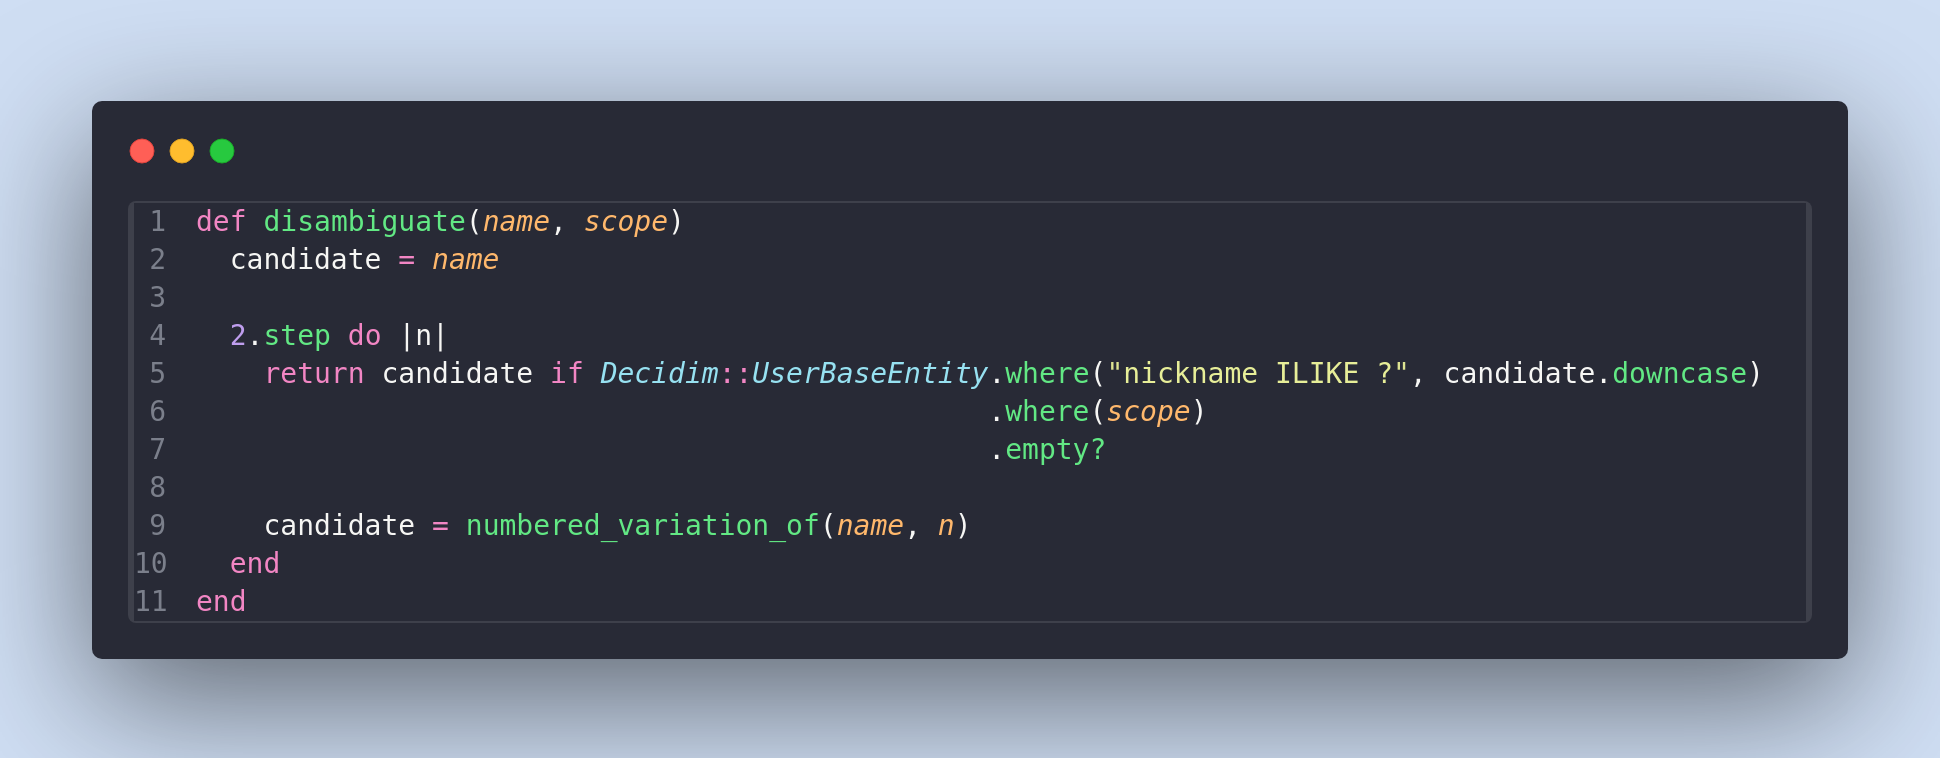
\includegraphics[width=\textwidth]{figuras/desambiguate-original.png}
  \fonte{Próprio autor}
\end{figure}

Ora, dado que inicialmente a desambiguação é case insensitive, e o \textit{nickname} candidato era transformado para minúsculo antes de realizar a consulta no banco, se o \textit{nickname} presente no banco também estivesse no mesmo \textit{case} do candidato, bastaria fazer uma comparação direta com o operador de igualdade \texttt{=}.
Para isso, foi utilizado o operador \texttt{LOWER} disponível no PostgreSQL para compor a consulta. A Figura \ref{fig:desambiguate-modificado} demonstra a nova versão do método de desambiguação com essa alteração.

\begin{figure}[htbp]
  \centering
  \caption{Código fonte do método desambiguação modificado}
  \label{fig:desambiguate-modificado}
  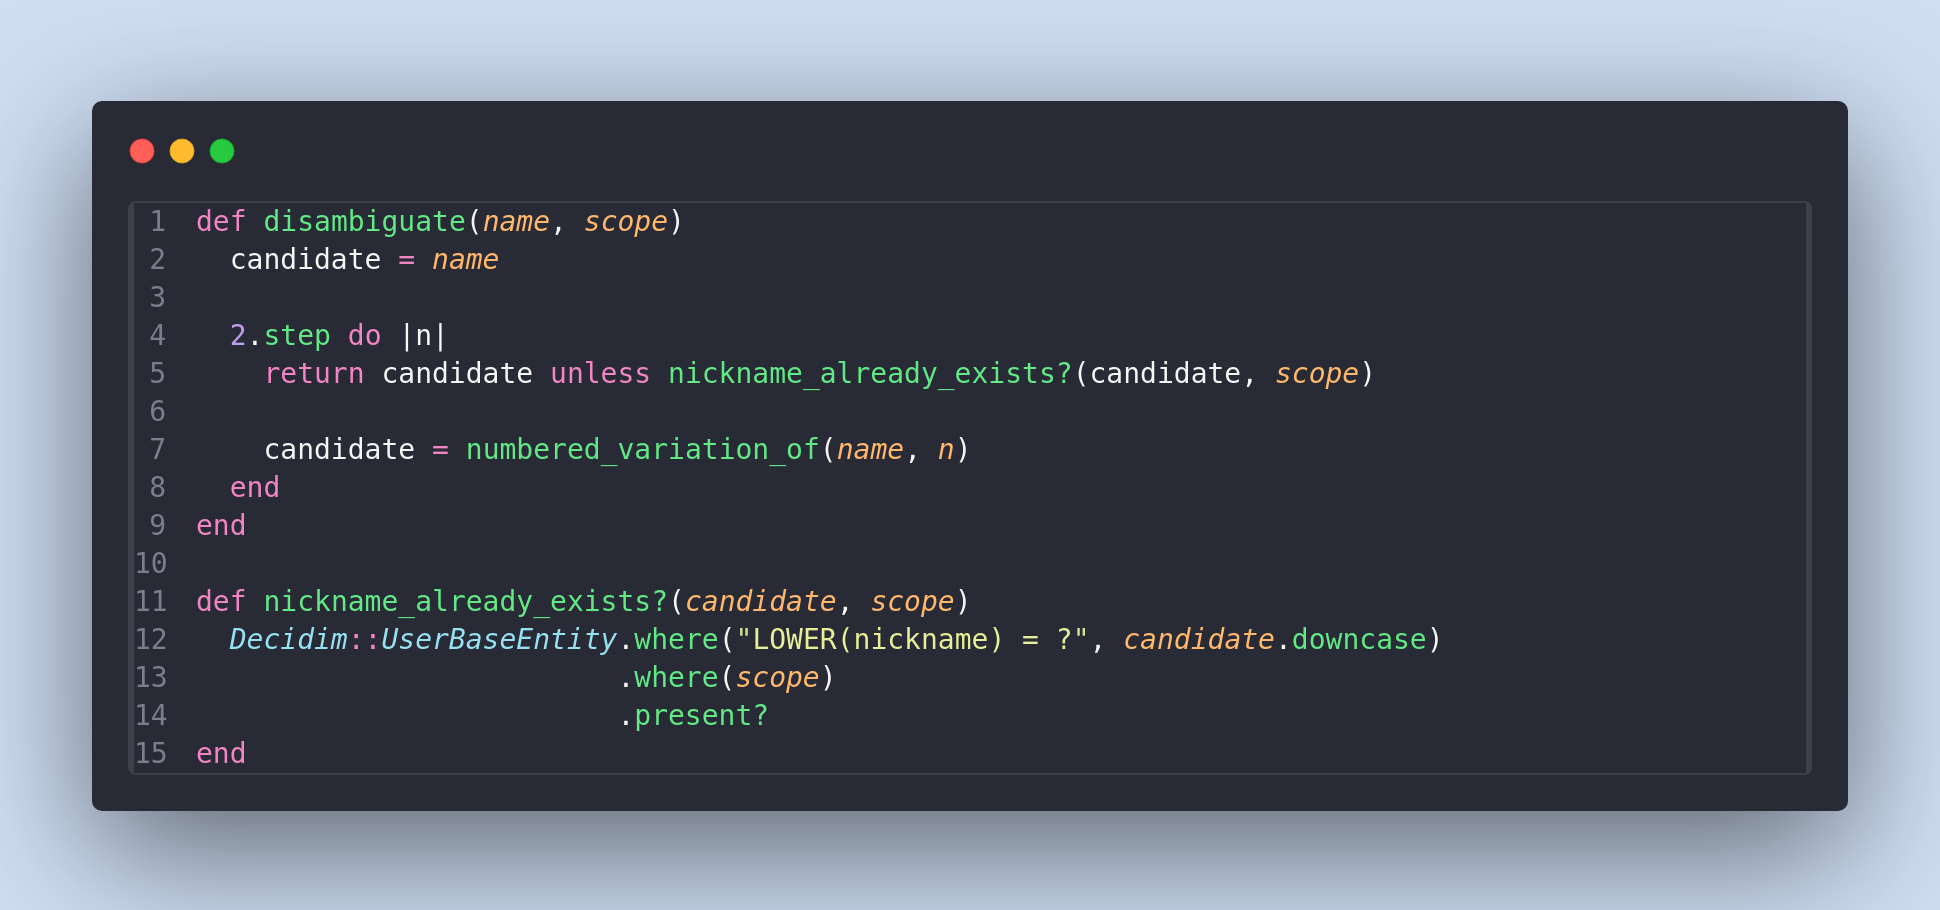
\includegraphics[width=\textwidth]{figuras/desambiguate-modificado.png}
  \fonte{Próprio autor}
\end{figure}

A fim de comparação, foi executado no ambiente produtivo do Brasil Participativo ambas consultas SQL utilizadas no método \texttt{disambiguate} com o comando \texttt{EXPLAIN ANALYZE}.
As consultas receberam um parâmetro extra \texttt{LIMIT 1} para não trazer todas as tuplas que satisfazem a condição. Isso foi necessário pois a ferramenta utilizada para executar a consulta no ambiente produtivo foi a \texttt{Rails DB}, que é executada no próprio \textit{frontend} da aplicação.

Na Figura \ref{fig:execucao-consulta-com-ilike} é mostrada a consulta executada no ambiente produtivo utilizando \texttt{ILIKE}, enquanto na Figura \ref{fig:execucao-consulta-com-lower} é mostrada a que utiliza \texttt{LOWER}.

\begin{figure}[htbp]
  \centering
  \caption{Consulta SQL com \textit{Explain Analyze} utilizando \texttt{ILIKE}}
  \label{fig:execucao-consulta-com-ilike}
  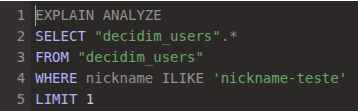
\includegraphics[width=\textwidth]{figuras/execucao-consulta-com-ilike.png}
  \fonte{Próprio autor}
\end{figure}

\begin{figure}[htbp]
  \centering
  \caption{Consulta SQL com \textit{Explain Analyze} utilizando \texttt{LOWER}}
  \label{fig:execucao-consulta-com-lower}
  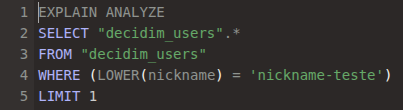
\includegraphics[width=\textwidth]{figuras/execucao-consulta-com-lower.png}
  \fonte{Próprio autor}
\end{figure}

Na Figura \ref{fig:consulta-com-ilike} é exibido o resultado da consulta utilizando \texttt{ILIKE}, e na Figura \ref{fig:consulta-com-lower} é exibido o resultado da consulta utilizando a comparação de igualdade com a função \texttt{LOWER}.
A plataforma no momento da consulta contava com mais de 1 milhão e 600 mil usuários.

\begin{figure}[htbp]
  \centering
  \caption{Resultado da consulta SQL com \textit{Explain Analyze} utilizando \texttt{ILIKE}}
  \label{fig:consulta-com-ilike}
  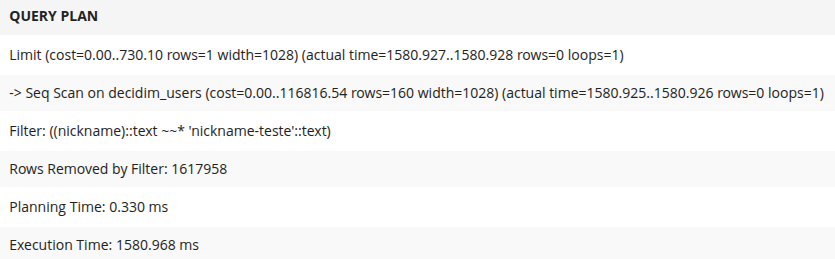
\includegraphics[width=\textwidth]{figuras/consulta-com-ilike.png}
  \fonte{Próprio autor}
\end{figure}

\begin{figure}[htbp]
  \centering
  \caption{Resultado da consulta SQL com \textit{Explain Analyze} utilizando \texttt{LOWER}}
  \label{fig:consulta-com-lower}
  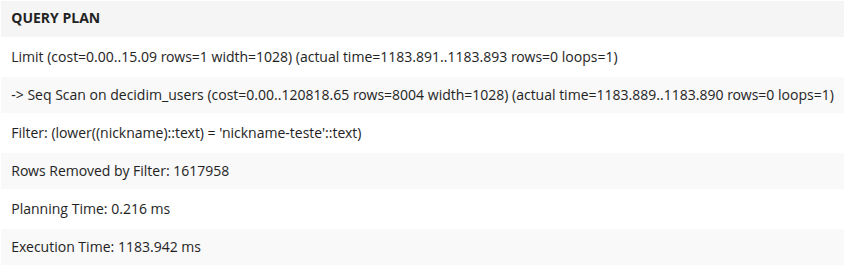
\includegraphics[width=\textwidth]{figuras/consulta-com-lower.png}
  \fonte{Próprio autor}
\end{figure}

Nota-se que a consulta que utiliza o \texttt{LOWER} gasta cerca de 25\% menos tempo para ser processada em comparação à consulta que utiliza o \texttt{ILIKE}.
Dado fato de que até o presente momento deste trabalho não houveram cenários de uso da plataforma na mesma escala que foi vista com o PPA em 2023, esta solução foi considerada como satisfatória. Mas, ainda existem pontos para serem explorados em futuras oportunidades, como por exemplo o uso de índices sobre o \textit{nickname} em \textit{lowercase}.

As modificações realizadas nessa \textit{sprint} estão disponíveis no \textit{merge request} em \url{https://gitlab.com/lappis-unb/decidimbr/decidim-govbr/-/merge_requests/41}